\ifnum \Version=1
\question[5] % 
Consider the differential equation $\displaystyle \dydt = -(y-k)^2(y-2)$, where $y$ is a real function of $t$, and $t \ge 0$, and $0<k<1$. The critical points are located at $y=k$ and $y=2$. 
\begin{parts}
    \part Draw the phase line, and determine whether the critical points (if any) are stable, semi-stable, or unstable. Please show your work. 
    \ifnum \Solutions=0 \vspace{8cm}\fi
    \part Using results from part (b) to sketch several solution curves in the $ty$-plane for $t \ge 0$. Don't forget to label your axes. 
\end{parts}
\ifnum \Solutions=1 {\color{DarkBlue} 
} 
\else 
\fi
\fi


\ifnum \Version=2
\ifnum \Solutions=0 \newpage \fi
\question[5] Solve the initial value problem and solve for $y$ to obtain an explicit expression for $y$ in terms of $t$. Please show your work.
$$\displaystyle t\,\frac{dy}{dt} + 3y =  36 t^{-2}e^{-t}, \ y(1) = 0, \quad t > 0$$.
\ifnum \Solutions=1 {\color{DarkBlue} \\[12pt] 
In standard form the DE is
$$\displaystyle \frac{dy}{dt} + \frac3t y =  36 t^{-3}e^{-t}$$
The integrating factor is
\begin{align}
    \mu = e^{\int 3/t \, dt} = e^{3 \ln t} = t^3
\end{align}
Multiplying by the integrating factor yields
\begin{align}
    t^3 \dydt + 3t^2 y &= 36e^{-t} \\
    \ddt \left( t^3 y \right) &= 36e^{-t} \\
     t^3 y  &= c_1 - 36e^{-t} 
\end{align}
When $t=1$, $y=0$, so
\begin{align}
    0 &= c_1 - 36/e \quad \Rightarrow \quad c_1 = 36/e
\end{align}
Thus
\begin{align}
    y = \frac{36}{e}t^{-3} - 36 t^{-3}e^{-t}
\end{align}
} 
\else 
\vspace{3cm}
\fi
\fi   



\ifnum \Version=3
\ifnum \Solutions=0 \newpage \fi
\question[5] Solve the initial value problem and solve for $y$ to obtain an explicit expression for $y$ in terms of $t$. Please show your work.
$$\displaystyle t\,\frac{dy}{dt} + 4y =  12 t^{-3}e^{2t}, \ y(1) = 2, \quad t > 0$$.
\ifnum \Solutions=1 {\color{DarkBlue} \\[12pt] 
In standard form the DE is
$$\displaystyle \frac{dy}{dt} + \frac4t y =  12 t^{-4}e^{2t}$$
The integrating factor is
\begin{align}
    \mu = e^{\int 4/t \, dt} = e^{4 \ln t} = t^4
\end{align}
Multiplying by the integrating factor yields
\begin{align}
    t^4 \dydt + 4t^3 y &= 12e^{2t} \\
    \ddt \left( t^3 y \right) &= 12e^{2t} \\
     t^4 y  &= c_1 + 6e^{2t} 
\end{align}
When $t=1$, $y=2$, so
\begin{align}
    2 &= c_1 + 6e^2 \quad \Rightarrow \quad c_1 = 2 - 6e^2
\end{align}
Thus
\begin{align}
    y = (2-6e^2)t^{-4} + 6t^{-4}e^{2t}
\end{align}
} 
\else 
\vspace{3cm}
\fi
\fi   





\ifnum \Version=4
\ifnum \Solutions=0 \newpage \fi
\question[5] Solve the initial value problem and solve for $y$ to obtain an explicit expression for $y$ in terms of $t$. Please show your work.
$$\displaystyle t\,\frac{dy}{dt} = 4t^2y +  6t^2e^{2t^2}, \ y(1) = 0, \quad t > 0$$
\ifnum \Solutions=1 {\color{DarkBlue} \\[12pt] 
In standard form the DE is
$$\displaystyle \frac{dy}{dt} - 4t y =  6 te^{2t^2}$$
The integrating factor is
\begin{align}
    \mu = e^{-\int 4t \, dt} = e^{-2t^2} 
\end{align}
Multiplying DE in standard form by the integrating factor yields
\begin{align}
    e^{-2t^2} \dydt - 4te^{-2t^2} y &= 6t \\
    \ddt \left( e^{-2t^2} y \right) &= 6t \\
     e^{-2t^2} y  &= c_1 + 3t^2
\end{align}
When $t=1$, $y=0$, so
\begin{align}
    0 &= c_1 + 3(1)^2 \quad \Rightarrow \quad c_1 = -3
\end{align}
Thus
\begin{align}
    y = -3 e^{2t^2} +3t^2e^{2t^2} = 3e^{2t^2}\left( t^2 -1 \right)
\end{align}
} 
\else 
\vspace{3cm}
\fi
\fi   





\ifnum \Version=6
\newpage
\question[4] Consider the DE $\displaystyle \dydt = y^2(12-y)$. 
\begin{parts}
    \part Sketch the phase line and classify the critical points according to their stability. 
    \ifnum \Solutions=1 {\color{DarkBlue} 

    \textbf{Solutions:} Setting $y'=0$ we find that the equilibrium points are $y = 0, 12.$ If we sketch the phase line we obtain the following.
    
    \begin{center}
        \begin{tikzpicture}[ultra thick]
        \DrawHorizontalPhaseLine[$y$]{0,12}{-0.5,6}{12.5}%
    \end{tikzpicture}
    \end{center}
    So $y=0$ is semi-stable, and $y=12$ is stable. 

} 
\else 
\vfill
\fi
    \part Determine the values of $y$ where the solution curves are concave up and where the curves are concave down. Please show your work. 
    
    \ifnum \Solutions=1 {\color{DarkBlue} 
        \textbf{Solutions:} If $f(y) = y'$, then $$\dydtt = \dfdy \, \dydt$$ Also 
        $$\dfdy = \ddy\left(12y^2-y^3\right) = 24y-3y^2 = 3y(8-y)$$
        So $df/dy = 0$ when $y=0$ and $y = 8$. There may be inflection points where either (or both) $df/dy$ and $dy/dt$ are zero. So there could be inflection points at $$y = 0, \ y = 8,\  y = 12$$ When both derivatives have the same sign, the solutions are concave up, and when they have opposite signs the solutions are concave down. 
        \begin{center}            
            \renewcommand{\arraystretch}{1.4}
            \begin{tabular}{c|cccc} 
            $ y $ & $(-\infty,0)$ & $(0,8)$ & $(8,12)$ & $(12,\infty)$ \\ \hline 
            $\displaystyle  dy/dt$ & $+$ & $+$ & $+$ & $-$ \\ \hline
            $ \displaystyle df/dy $ & $-$ & $+$ & $-$ & $-$  \\[4pt] \hline
            $ \text{concavity} $ & \text{down} & \text{up} & \text{down} & \text{up}\\ \hline
            \end{tabular}
        \end{center}  
        So concave up on $0<y<8$ and $12<y$. Concave down otherwise. 
} 
\else 
\vfill
\newpage
\fi    
\end{parts}

\fi 



\ifnum \Version=7
\newpage
\question[4] Consider the DE $\displaystyle \dydt = y(4-y^2)$. 
\begin{parts}
    \part Sketch the phase line and classify the critical points according to their stability. 
    \ifnum \Solutions=1 {\color{DarkBlue} 

    \textbf{Solutions:} Setting $y'=0$ we find that the equilibrium points are $y = 0, \pm 2.$ If we sketch the phase line we obtain the following.
    
    \begin{center}
        \begin{tikzpicture}[ultra thick]
        \DrawHorizontalPhaseLine[$y$]{-2,0,2}{-3,1}{-1,3}%
    \end{tikzpicture}
    \end{center}
    So $y=0$ is un-stable, and $y=\pm 2$ is stable. 

} 
\else 
\vfill
\fi
    \part Determine the values of $y$ where the solution curves are concave up and where the curves are concave down. Please show your work. 
    
    \ifnum \Solutions=1 {\color{DarkBlue} 
        \textbf{Solutions:} If $f(y) = y'$, then $$\dydtt = \dfdy \, \dydt$$ Also 
        $$\dfdy = \ddy\left(4y-y^3\right) = 4-3y^2 $$
        So $df/dy = 0$ when $y= \pm \sqrt {4/3} = \pm \frac{2}{\sqrt 3}$. There may be inflection points where either (or both) $df/dy$ and $dy/dt$ are zero. So there could be inflection points at $$y = 2, -\frac{2}{\sqrt 3},0,\frac{2}{\sqrt 3} , 2$$ When both derivatives have the same sign, the solutions are concave up, and when they have opposite signs the solutions are concave down. 
        \begin{center}            
            \renewcommand{\arraystretch}{1.4}
            \begin{tabular}{c|cccccc} 
            $ y $ & $(-\infty,-2)$ & $(-2,-\frac{2}{\sqrt 3})$ & $(-\frac{2}{\sqrt 3},0)$ & $(0,\frac{2}{\sqrt 3})$ & $(\frac{2}{\sqrt 3},2)$ & $(2,\infty)$ \\ \hline 
            $\displaystyle  dy/dt$ & $+$ & $-$ & $-$ & $+$ & $+$ & $-$\\ \hline
            $ \displaystyle df/dy $ & $-$ & $-$ & $+$ & $+$ & $-$ & $-$\\[4pt] \hline
            $ \text{concavity} $ & \text{down} & \text{up} & \text{down} & \text{up} & \text{down} & \text{up}\\ \hline
            \end{tabular}
        \end{center}  
} 
\else 
\vfill
\newpage
\fi    
\end{parts}

\fi 